\scanpage{30}
\uline{Dém} En deux étapes

\uline{LEMME 1} $\xi_k=0$ si \inserted{$k\geq N$ tel que} $c_{i,k-i}\not\equiv0\ (p)$

\uline{Lemme} 1.1. Soient \deleted{$\unsure{k,k'}$} $k'\geq k\geq N$ tels que, posant $j=k-i$, $j'=k'-i\unsure{\deleted{j}|^\ast}$, on ait
\[
(4)\qquad c_{i,j}\not\equiv0\ (p)\quad\text{et}\quad c_{i,j'}\not\equiv0\ (p)
\]
Alors on a l'équivalence
\[
(5)\qquad c_{j'-j,j}\not\equiv0\ (p)\quad\Longleftrightarrow\quad c_{j'-j,j+\unsure{i|j}}\not\equiv0\ (p)
\]
et si les conditions équivalentes (5) sont satisfaites, on a l'équivalence
\[
(6)\qquad\xi_k=0\quad\Longleftrightarrow\quad\xi_{k'}=0.
\]

\uline{Dém de} 1.1. Calculons dans $\mathbf Q$
\[
\text{(a)}\quad c_{j'-j,j+i}/c_{j'-j,j}=\frac{(j'+i)!}{\deleted{(j'-j)!}(j+i)!}:\frac{(j'\deleted{+\unsure{i|j}})!}{\deleted{(j'-j)!}j!}
\]
\margin{$\unsure{\alpha\ //}$}
\[
\text{(b)}\quad c_{i,j'}/c_{ij}=\frac{(i+j')!}{\deleted{i!}j'!}:\frac{(i+j)!}{\deleted{i!}j!}
\]
\deleted{\[
\text{(b)}\quad c_{ij'}/c_{ij}=\frac{(i+j')!}{i!j'!}:\frac{(i+j)!}{i!j!}
\]
le quotient de (a) et (b) \unsure{est}, grâce à (4)
\[
(i+j)!\sim i!j!\qquad(i+j')!\unsure{\simeq|\sim}i!j'!
\]
donc le premier \unsure{mb.} de (a) est égal à
\[
\frac{i!j'!}{i!j!}:\frac{(j'+i-j)!}{\unsure{i!}}=
\]}
\margin{\deleted{Or dans $\mathbf Z_p$ pour ce rel. de divisibilité, on}}
\figure{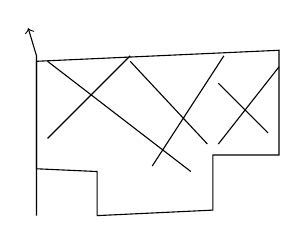
\begin{tikzpicture}[scale=.7]
\draw[->] (0,0)--(0,2.9)--(-.15,3.4);
\draw (0,2.8)--(4.4,3)--(4.4,1.1)--(3.2,1.1)--(3.2,.1)--(1.1,0)--(1.1,.8)--(0,.85)--cycle;
\draw (.2,2.8)--(2.8,.8) (.2,1.4)--(1.7,2.9) (1.7,2.8)--(3.1,1.3) (2.1,.9)--(3.4,2.9) (3.3,2.4)--(4.2,1.5) (3.3,1.3)--(4.4,2.7);
\end{tikzpicture}}
Donc les deux quantités (a) et (b) sont \unsure{égaux|égales}, et comme (b) est un quotient de deux unités \deleted{p-adiques} \inserted{de $\mathbf Z_p$}, on voit que $c_{j'-j,j+i}$ et $c_{j'-j,j}$ sont \unsure{équivalents|équivalent} pour la divisibilité, donc l'un est une \unsure{unité|unit} ssi l'autre l'est. Quand il en est ainsi, la
\mspage{29}
